\documentclass[14pt]{extarticle}
\usepackage[utf8]{inputenc}
\usepackage{longtable}
\usepackage{graphicx}
\usepackage{verbatim}
\usepackage{multirow}
\usepackage{amsmath,amsthm,amssymb}
\usepackage[utf8]{inputenc}
\usepackage[russian]{babel}
\graphicspath{ {images/} }

\title{Распознавание эмоций человека по речи}
\author{Айдар Мусин\\Научный руководитель: Максим Таланов}
\date{Июнь 2015, Университет Иннополис}

\begin{document}

\begin{titlepage}
\maketitle
\end{titlepage}

\tableofcontents
\begin{abstract}
	Технология распознавания эмоций человека по речи может быть использована во многих интересных областях. Не удивительно, что существует множество исследований на эту тему. В этой статье рассматриваются исследования по распознаванию эмоций в речи. Выделяются отличия некоторых подходов и раскрываются плюсы и минусы этих подходов. Затем, на основе проанализированной информации предлагается реализация упрощенной системы распознавания базовых эмоций
\end{abstract}

\section{Введение}
Люди выражают эмоции не только с помощью жестов и мимики. Эмоции также выражаются в речи. Когда человек, например, возбужден, тон голоса становиться выше, растет темп речи и средняя длительность слогов уменьшается. Такого рода характеристики, связанные с эмоциями описаны во многих исследованиях в этой области.
Мы способны распознавать базовые эмоции независимо от языка, возраста и пола говорящего. Это означает, что существует связь между динамикой звуковых характеристик и выражаемыми эмоциями. И это доказывает множество работ. Значит, возможно реализовать такую технологию распознавания эмоций, которая работает независимо от языка, возраста и пола говорящего.

Почему такого рода технология может быть полезна? На самом деле, данное решение может быть использовано во многих областях. Наиболее из очевидных из которых: при построении роботов и для оценки качества обслуживания клиентов.
Для роботов, которые работают в социальной среде, может оказаться важной и необходимой такая способность. Это относиться к теме эмоциональных вычислений. 
Эмоциональные вычисления (affective computing) это изучение и развитие систем и устройств, которые способны распознавать, интерпретировать и имитировать человеческие эмоции. Этот подход к разработке роботов выделяет важность эмоций и доказывается важностью эмоций для людей. Потому что эмоции помогают лучше взаимодействовать людям, эмоциональная окраска позволяет улучшить запоминание, также это помогает при принятии решений.
Во-первых, технология распознавания эмоций может улучшить систему принятия решений. Так как могут возникать ситуации, когда роботу для принятия решения необходимо учитывать эмоциональное состояние человека. К тому же, выявление связей между звуковыми характеристиками и эмоциями, дает возможность реализовать эмоциональную речь робота. Если у говорящего робота будет способность эмоционально окрашивать некоторые выражения, это позволит ему лучше взаимодействовать с людьми. В целом, можно сделать вывод, что робот с возможностью распознавания и имитации эмоций более дружелюбен и эффективен. Уже существуют такие роботы, например, робот Pepper:
\begin{quote}
	Pepper это первый робот, спроектированный для жизни с людьми. К сожалению, он не убирается, не готовит и не имеет супер возможностей. Pepper – социальный робот, способный поговорить с Вами, распознавать и реагировать на ваши эмоции, способный передвигаться и существовать автономно.\cite{pepper}
\end{quote}
Более приближенное к настоящему применение этой технологии лежит в области оценки качества обслуживания клиентов. Например, call-центры ведут записи звонков, и для оценки качества работы операторов, можно анализировать звонки и выявлять особо эмоциональные разговоры. Эта технология может быть использована вместе с распознаванием речи. И для распознавания эмоций говорящего, можно анализировать звуковые характеристики и произнесенные фразы.
%%%%%%%%%%%%%%%%%% Examples!!!!!!!!!!!!!!!

\section{Цель работы}

Существует много работ рассматривающих распознавание эмоций по речи. Их основные отличия в использовании различных:
\begin{itemize}
	\item Акустических характеристик
	\item Признаков
	\item Методов классификации
	\item Распознаваемы эмоции
\end{itemize}

Существует много работ рассматривающих распознавание эмоций по речи. Их основные отличия в использовании различных: акустических характеристик, признаков, методов классификации, распознаваемых эмоций.
Также существуют статьи, в которых рассматриваются эти отличия, но зачастую в них рассматриваются только акустические характеристики, признаки и методы классификации. Не часто рассматривается, например, влияние на точность распознаваемые эмоции.
Таким образом, главная цель этой работы рассмотреть отличия различных подходов и разработать упрощенный прототип распознавания эмоций по речи. Затем, проверить влияние различных параметров на точность распознавания. Также, рассмотреть способы решения таких проблем как: извлечение звуковых характеристик, удаление шума, разбиение речи на фразы. Будут рассмотрены конкретные библиотеки и алгоритмы для решения этих проблем.

\section{Обзор}
\subsection{Акустические характеристики}
Голос, как и любой другой звук может быть описан некоторыми акустическими характеристиками. Перед тем рассматривать конкретные исследования, стоит рассмотреть эти акустические характеристики:
\begin{itemize}
	\item Тон или фундаментальная частота
	\item Громкость
	\item Форманта
	\item Мел-кепстральные коэффициенты
\end{itemize}

\subsubsection{Высота тона}
Частота человеческого голоса находиться в области между 300 и 3400 Гц. А фундаментальная (основная) частота  для мужского пола между 85 и 185 Гц, а для женского пола между 165 и 255 Гц.
\begin{quote}
Основная частота- частота повторения для периодической функции, определяется (нестрого) как низшая частота сложной периодической волны, иногда называется первой гармоникой  \cite{wiki1}.
\end{quote}

\subsubsection{Громкость}
Эта характеристика звука также может быть полезна для распознавания эмоций по речи. Но стоит отметить, что необходимо работать с ней с осторожностью, ведь эта характеристика очень сильно зависит от качества записи, от специфичной манеры говорить и других факторов, которые могут способствовать получению ложных данных.
\begin{quote}
Гроомкость звука — субъективное восприятие силы звука (абсолютная величина слухового ощущения). Громкость главным образом зависит от звукового давления ичастоты звуковых колебаний. Также на громкость звука влияют его спектральный состав, локализация в пространстве, тембр, длительность воздействия звуковых колебаний и другие факторы \cite{wiki_loudness}
\end{quote}

\subsubsection{Форманта и мел-кепстральнаые коэфициенты}
Часто для распознавания эмоций достаточно тона и громкости голоса. Но для более точных результатов можно использовать и другие характеристики звука. Например, форманты или мел-кепстральные коэффициенты. 
\begin{quote}
Formant is a range of frequencies of a complex sound in which there is an absolute or relative maximum in the sound spectrum". In speech science and phonetics, however, a formant is also sometimes used to mean an acoustic resonance of the human vocal tract.\cite{wiki2}
\\
\\
In sound processing, the mel-frequency cepstrum (MFC) is a representation of the short-term power spectrum of a sound, based on a linear cosine transform of a log power spectrum on a nonlinear mel scale of frequency\cite{wiki3}.
\end{quote}


\subsection{Признаки}
Для классификации эмоций используя акустические характеристики речи, необходимо сначала выделить признаки и закономерности этих среди этих характеристик. Таким образом, из обучающей выборки мы вычисляем признаки для каждой эмоции. И когда уже классификатор обучен, классификация проходит следующим образом:
\begin{enumerate}
	\item извлечь признаки из обрабатываемой записи
	\item сравнить эти признаки с признаками определенных эмоций
\end{enumerate}

По тому, как и для кого рассчитываются эти признаки, их можно разделить на две группы: 
\begin{itemize}
	\item зависимые от говорящего
	\item независимые от говорящего
\end{itemize}

\subsubsection{Speaker-dependent features}
Зависимые от говорящего признаки рассчитываются для каждого человека отдельно. Поэтому требуется разделенная обучающая выборка. И при классификации необходимы идентификация человека и рассчитанные признаки для его речи. Во время классификации сравниваются полученные признаки с его персональными признаками. Данный подход может оказаться более точным, потому что в отличие от другого подхода, здесь нет такого большого разброса значений. Но данный подход не универсален, поскольку необходимо для каждого человека хранить статистические данные (признаки). Эти признаки основаны на некоторых средних значениях, например, средняя высота тона, средняя громкость, средний диапазон высоты тона и т.д., а эти значения разные для всех людей. Поэтому такие признаки могут быть применены в очень редких случаях.
\subsubsection{Speaker-independent features}
В отличие от предыдущего подхода разделенная обучающая выборка не требуется. Но поскольку точность классификации сильно зависит от обучающей выборки, она должна содержать как можно больше записей с как можно разными людьми (пол, возраст, родной язык). Эти признаки основаны на динамике акустических характеристик и некоторых средних значениях.


\subsection{Классификация}
С одной стороны, проблема классификации в этом случае очень похожа на другие случаи и может быть решена с помощью таких классификаторов как: Бинарная диаграмма решений, Наивный Байесовский классификатор, Нейронные сети, Векторная Машина.
Но с другой стороны, присутствуют некоторые специфичные моменты, вызванные похожестью некоторых эмоций и неоднозначностью между ними. Большинство методов классификации очень подробно рассмотрены в статье
 \cite{SirishaSirvinasSiva}. Давайте рассмотрим некоторые из них.
\subsubsection{Бинарная диаграмма решений}
Бинарное дерево принятия решения - это структура данных, которая используется для представления булевой функции. Булева функция может быть представлена как направленный ацикличный граф, состоящий из внутренних узлов решений, каждый из которых имеет по два потомка, и терминальных узлов, каждый из которых соответствует одному из значений булевой функции.
\\
\\
\emph{Достоинства:} легкая реализация, четка видна связь между входными и выходными данными. Обучение и классификация простые и быстрые. Точность сравнима с другими классификаторами на простых данных. Возможность преобразовать в простые правила классификации.
\\
\\
\emph{Недостатки:} при обучении могут получиться слишком сложные деревья, которые не обобщают реальные данные. Проблема построения оптимального дерева – NP полная проблема. Алгоритмы обучения построены на эвристических алгоритмах таких как жадные алгоритмы. Где на каждом шаге принимается локальное оптимальное решение. Такие алгоритмы не обязательно приводят к глобально оптимальным решениям.
\\
\\
\subsubsection{Искусственные нейронные сети}
Искусственные нейронные сети – математическая модель, а также её программное или аппаратное воплощение, построенная по принципу организации и функционирования биологических нейронных сетей — сетей нервных клеток живого организма
\\
\\
\emph{Advantages:} Neural systems are rather easy to implement (you do not need a good linear algebra solver as for examples for SVNs). Neural networks often exhibit patterns alike to those exhibited by humans. Although this is more of interest in cognitive sciences than for functional examples.
\\
\\
\emph{Disadvantages:} Long preparing time, Neural systems can't be retrained. Provided that you include information later, this is just about difficult to add to an existing system. Taking care of time arrangement information in neural systems is an exceptionally confounded point.
\\
\subsubsection{Naïve Bayes classifier}
The Naive Bayes Classifier procedure is reliant upon the purported Bayesian hypothesis and is particularly suited when the dimensionality of the inputs is high. Notwithstanding its effortlessness, Naive Bayes can frequently outflank more refined grouping strategies.
\\
\\
\emph{Advantages:} fast to train (single scan). Fast to classify Not sensitive to irrelevant features Handles real and discrete data Handles streaming data well.
\\
\\
\emph{Disadvantages:} assumes independence of features



\subsection{Распознаваемые эмоции}
Точность распознавания эмоций зависит не только от выделенных признаков и методов классификации, это также зависит от распознаваемых эмоций. Это вызвано тем, что некоторые эмоции выражаются очень похожим образом. Чем больше будет выбрано эмоций для распознавания, тем, скорее всего, будет меньше точность их распознавания. Поэтому это некий компромисс между количеством распознаваемых эмоций и точностью.
\begin{figure}[t]
	\centering
	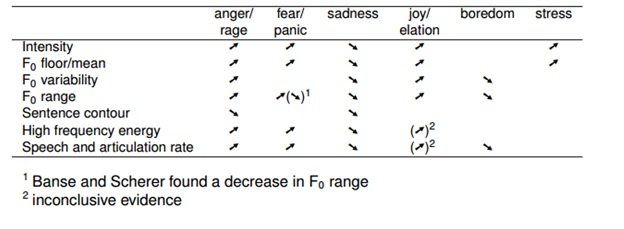
\includegraphics[scale=0.8]{emotion-table-example}
	\caption{Sound characteristics for emotions [1]}
	\label{fig:emotion-table-example}
\end{figure}

Например, на рис. 1 показана связь между эмоциями и некоторыми признаками акустических характеристик. Видно, что некоторые эмоции очень похожи по некоторым показателям (злость-радость, грусть-скукота). Хотя и количество эмоций не такое большое, уже можно видеть некоторые пересечения в признаках. С увеличением количества эмоций, таких пересечений станет только больше. Поэтому важно определять набор распознаваемых эмоций для каждой решаемой задачи отдельно.
\subsection{Тенденции последних исследований}
Большинство работ в этой области все больше и больше используют признаки, независящие от говорящего. Выделяя из речи признаки, основанные на динамике речевого сигнала. Поскольку такой подход более универсален и может быть применен во многих отраслях.

Проблема классификации часто решается с использованием: векторных машин, алгоритма классификации ближайшего соседа, скрытых Марковских моделей и нейронных сетей. Хотя более простые методы, такие как: бинарные диаграммы решения, нечеткие множества тоже работают и обладают сравнимой точностью и эффективностью.

\begin{table}[h]
	\small
	\begin{tabular}{|p{3cm}|p{3cm}|p{3cm}|p{3cm}|p{3cm}|}
		Название & Авторы & Использованные акустические характеристики и признаки & Методы классификации & Распознаваемые эмоции \\ \hline
		Real-time automatic emotion recognition
		from speech & Britta Wrede, Elisabeth André & pitch, loudness, spectrum, MFCC, speaking rate. DDS, mean, median, varince values for characteristics & SVM, Naive Bayes & positive-active, negative-active, positive-passive, negative-passive\\ \hline
		The production and recognition of emotions in
		speech: features and algorithms & Pierre-Yves Oudeyer & pitch, loudness. Mean, variance, contour rising or falling features. & k-NN, SVM, Naive Bayes& Calm, anger, sadness, comfort, happiness\\ \hline
		Speech Emotion Recognition Using Hidden Markov Models & Albino Nogueiras, Asunción Moreno, Antonio Bonafonte, and José B. Mariño & pitch, energy & Hidden Markov Models & Surprise, Joy, Anger, Fear, Disgust, Sadness, Neutral \\\hline
	\end{tabular}
	\caption{Comparison of some studies}
	\
\end{table}
\section{Реализация}
\subsection{Постановка задачи}
Главной задачей является разработать прототип системы распознавания эмоций по речи, который можно будет в дальнейшем усовершенствовать. Программа должна быть способна распознавать эмоции по речи, считываемой с микрофона или с звукового файла. Также, распознавание должно быть в какой-то мере устойчиво к лишним шумам. Для реализации был выбран язык C\#, а также библиотеки для работы со звуком, которые будут описаны дальше.

Разработка нашей системы может быть разделена на 4 этапа:
\begin{enumerate}
	\item разработка модуля получения акустических характеристик с звукового файла или микрофона
	\item разработка модуля разбиения речи на фразы или слова
	\item разработка модул получения признаков
	\item построение классификатора
\end{enumerate}

\begin{figure}
	\centering
		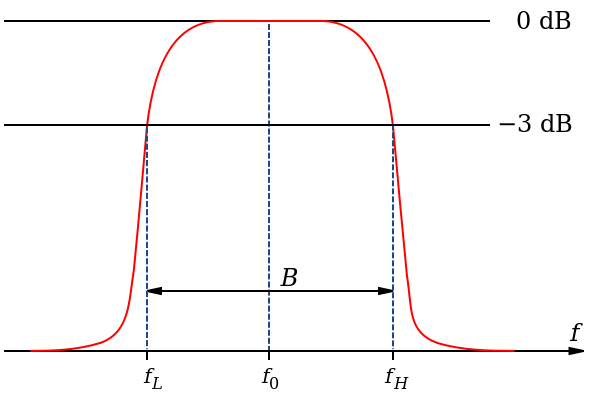
\includegraphics[scale=0.7]{images/pass-band-filter.png}
	\caption{Полосовой фильтр}
	\label{fig:pass-band-filter}
\end{figure}

\subsubsection{Модуль получения акустических характеристик}

Во-первых, для получения точных характеристик голоса, необходимо предварительно отфильтровать запись. Это позволит, не только избежать ложных результатов, но и позволит выявить промежутки молчания в речи. Что в свою очередь обеспечит возможность разбиения речи на фразы.
\\

Для получения неотфильтрованных характеристик можно использовать библиотеки:
\begin{itemize}
	\item NAudio (http://naudio.codeplex.com)
	\item Bass Audio library (http://www.un4seen.com/)
\end{itemize}

С помощью этих библиотек можно получать характеристики, например, используя Быстрое преобразование Фурье. Но они не поддерживают функции фильтрации, поэтому также придётся реализовывать фильтр. Простейший фильтр для человеческой речи может быть реализован в виде полосового фильтра.
Полосовой фильтр (рис. 2) - простейший фильтр, у которого выставляется полоса пропускания. И если значение не попадает в эту полосу (интервал), то оно игнорируется. 
\\
Для анализа речи также часто применяется программный пакет - PRAAT \cite{praat}. Библиотека имеет большой набор функций, в том числе и необходимые для нашей реализации:
\begin{itemize}
	\item Получние высоты основного тона
	\item Получение громкости
	\item Анализ спектрограммы
	\item Получение формант
	\item Функции фильтрации
\end{itemize}
Для фильтрации будем использовать встроенные функции удаления шума и полосовой фильтр.
Для работы с звуковыми файлами пакет имеет свой скриптовый язык. Работа с языком рассматриваться здесь не будет, поскольку описание можно найти на сайте разработчиков. 



Таким образом, используя пакет PRAAT, мы получаем ряд характеристик из звукового файла:
\begin{itemize}
	\item Основная высота тона (F0)
	\item Громкость (Intensity)
	\item Форманты (F1, F2, F3)
	\item Центр тяжести спектрограммы
\end{itemize}
Пример графика характеристик показан на рис. 3. Можно заметить, что есть интервалы, где все значения равны нулю - это результат работы фильтра. Полосовой фильтр установлен в соответствии с рамками человеческой речи, а функции удаления шума позволяют убирать различного рода артефакты, такие как белый шум. Таким образом, в результате фильтрации мы можем выявить интервалы молчания.
\begin{figure}
	\centering
		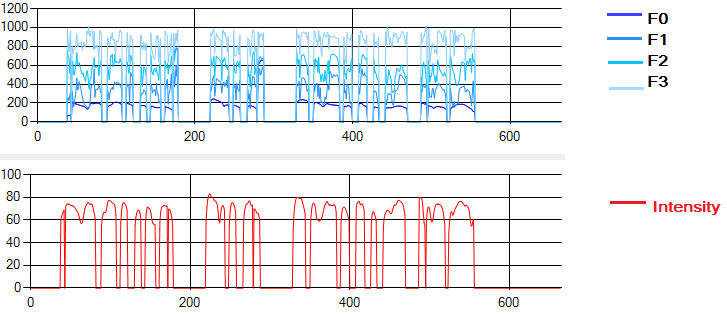
\includegraphics[scale=0.8]{images/sound-characteristics.png}
	\caption{Полученные акустические характеристики}
	\label{fig:sound-characteristics}
\end{figure}

\subsubsection{Разбиение речи на фразы}

Когда люди разговаривают, они придают различные эмоциональные окраски фразам путем изменения акустических характеристик. Поэтому для точного распознавания необходимо анализировать фразы отдельно.
Стоит отметить, что точное разбиение речи на фразы невозможно без фильтрации. Поэтому успех на этом этапе сильно зависит от предыдущего, где выявляются интервалы молчания. Затем, для разбиения речи на фразы можно применить простой алгоритм слияния:
 \begin{itemize}
	 \item Пока не встретился нуль, собираем данные фразы
		\item Как только встретился нуль, закрываем текущую фразу и начинаем собирать следующую.
 \end{itemize}

Но с этим простым алгоритмом могут возникнуть проблемы, если среди фразы возникнет нулевое значение. Эту проблему можно решить, если установить минимальную длину между фразами.
На рис. 4 показан результат разбиения речи на фразы, и видно, что внутри фраз тоже есть промежутки молчания, но они незначительные. 

Как результат после выполнения двух первых шагов, на выходе мы получаем ряд акустических характеристик и указатели на отдельные фразы. Теперь необходимо выделить признаки для дальнейшей классификации.
\begin{figure}
	\centering
		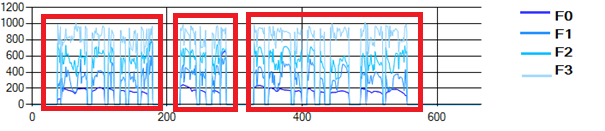
\includegraphics[scale=1]{images/phrases.png}
	\caption{Speech divided to phrases}
	\label{fig:phrases}
\end{figure}


\subsection{Получение признаков}

\begin{table}

\begin{tabular}{|p{2.2in}|p{2.2in}|} 
\hline
\multirow{3}{*}{Pitch (F0) }& Variance \\ \cline{2-2}
													& Range \\ \cline{2-2} 
													& DDS \\ \hline 
Formant 1 (F1) & DDS \\ \hline 
Formant 2 (F2) & DDS \\ \hline 
Formant 2 (F3) & DDS \\ \hline 
\multirow{3}{*}{Loudness (Intensity) } & Variance \\ \cline{2-2}
																		& Range \\ \cline{2-2}
																		& DDS \\ \hline 
\multirow{2}{*}{Time} & mean phrase duration \\ \cline{2-2} 
 & mean silence duration \\ \hline 
Spectrogramm & Center of gravity (centroid) \\ \hline 
\end{tabular}
	\caption{Using features}
	\label{Using features}
\end{table}

На предыдущих этапах мы получили ряд характеристик: высота основного тона, громкость, форманты, центр тяжести спектрограммы. Будем использовать признаки независящие от говорящего, значит, в первую очередь необходимо выделять динамику характеристик. Рассмотрим признаки, которые мы использовали: \\ \\
\emph{Вариативность.} Этот признак может быть расчитан с помощью стандартного отклонения:
\begin{center}
\[V=\sqrt{
\sum_{i=0}^{n}{
               (x_i-\overline{x})^2
               }
}
\]
 где  $\overline{x}$ среднее арифметическое множества \\
\end{center}
\emph{Диапазон.} Это разница между максимальным и минимальным значением.
\\\\
\emph{DDS (Difference-Distance-Slope)} Идея этого признака взята из статьи\\ \cite{brittaelizabet} \\ DDS вычисляется отдельно для каждой фразы (пример на рис. 5), затем для всей речи рассчитываются средние значения. Алгоритм обработки каждй фразы:
\begin{itemize}
	\item Найти $maximum$ и $minimum$ элементы для фразы
	\item $difference=maximum-minimum$
	\item $distance=maximum_{position}-minimum_{position}$
\end{itemize}

\begin{figure}
	\centering
		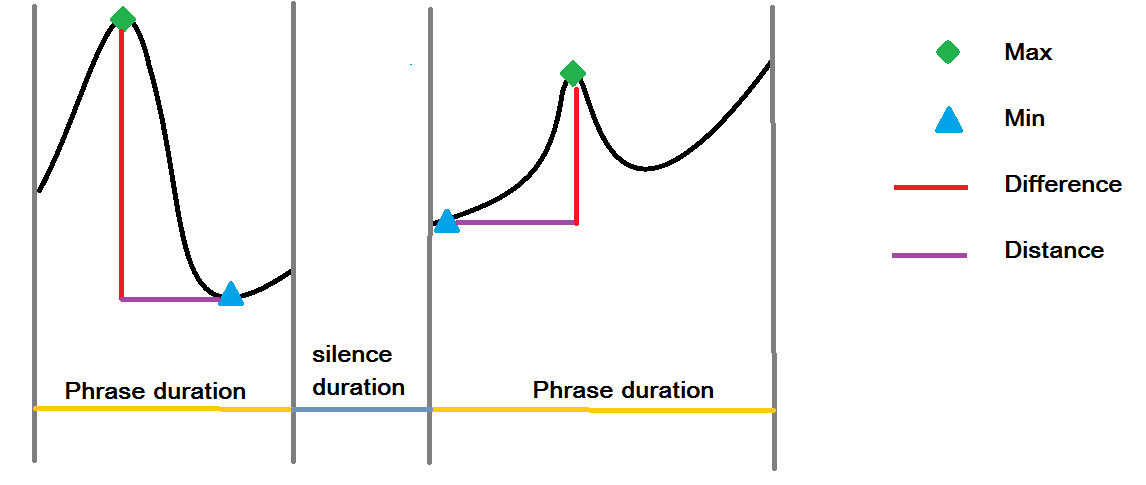
\includegraphics[scale=0.5]{images/dds.png}
	\caption{DDS}
	\label{fig:dds}
\end{figure}
Затем на основе указателей фраз рассчитываем среднюю длину фраз и длину интервалов молчания. Также расчет центра тяжести спектрограммы предоставляет пакет PRAAT. Таким образом, мы получаем набор признаков (табл. 2), который может описывать человеческую речь.
\subsection{Features from training data set}
For further building a classifier is necessary to identify relations between these features and emotions. It requires a training set with split emotional speech records. 

But before, should be selected emotions for recognition. A recognizable set of emotion is important for the system's accuracy. In this work will be used four emotions: \emph{anger, happiness, sadness and neutral}. Because these emotions are basic and they are more clearly expressed in human speech.

There are many databases of emotional speech. And they differ in:
\begin{itemize}
	\item number of emotions
	\item number of actors (speakers)
	\item nature of emotion (artificially played or really expressed emotions)
	\item number of various texts
\end{itemize}
"EmoDB"\cite{emodb} - german database of emotions will be used. It consists of emotional records spoken by 10 different actors. They express 7 emotions (anger, boredom, disgust, fear, happiness, sadness, neutral), but we will use only four emotions which we selected above. Each actor expresses an emotion with several texts. For our goals this database contains more than 250 speech records. About 70\% of records used as a training set, the rest will be used for testing. For each speech we calculated features, and for selected emotions was taken medians for each feature. So results of extracted features from training data set are represented in the Table 3.
\begin{table}[h]
	\centering
		\begin{tabular}{l|l|l|l|l|}
			\hline
				Feature/Emotion& anger&	happy	&sadness	&neutral\\ \hline
PitchDIf        & 146,70  & 172,125      & 61,85    & 95,51  \\ \hline
PitchDis        & -3,08 & -5,85 & -3,98 & -6,16 \\ \hline
IntDif          & 21,41  & 22,51      & 16,86  & 18,37  \\ \hline
IntDis          & 2,91 & 2,25         & -5,1         & -2,57 \\ \hline
F1Dif           & 233,4  & 201,835      & 149,50  & 196,46  \\ \hline
ddsF1Dis        & -0,4         & -5,2         & -4,52 & -3           \\ \hline
F2dif           & 323,44       & 332,025     & 317,41     & 312,08  \\ \hline
F2Dis           & -1,42 & -2,16 & 1,5          & -2           \\ \hline
F3Dif           & 343,18       & 359,926      & 334,083      & 425,46       \\ \hline
F3Dis           & -0,77 & 0,66  & 2,8          & 2,66  \\ \hline
PitchRange      & 680,54       & 505,09       & 392,145      & 430,9        \\ \hline
IntRange        & 31,61        & 30,17        & 28           & 27,24        \\ \hline
PitchVariance   & 9237,37  & 9671,95  & 3276,06  & 3858,43  \\ \hline
IntVariance     & 46,19  & 41,09  & 32,68  & 33,25  \\ \hline
PhraseDuration  & 28           & 30           & 22,01  & 27,25        \\ \hline
SilenceDuration & 6,5          & 5,5          & 17,46  & 6            \\ \hline
Centroid        & 578,32       & 495,88       & 212,815      & 340,67       \\ \hline
 \hline
		\end{tabular}
	\caption{Extracted features from training data set. Dif-Difference, Dis-Distance, Int-Intensity}
	\label{tab:ExtractedFeaturesFromTrainingDataSet}
\end{table}

\subsection{Classification}
So we have got some feature values for each emotion, and is needed to build classifier using them. Each feature has 4 values which mapped with emotions. Therefore, each emotion can be characterized by set of approximate values of features. For example, PitchDiff has values: 	137,08;  211,55; 67,32; 64,63; 

Problem here is how to identify that some value is closer to one of the feature's value. It is impossible to set strict confines of feature's
values for each emotion. In addition, some feature values are very similar and it's difficult divide them to four classes. But often among these 4 values exist two high and two low values. It caused by fact that some emotion very similar with some features, but they have some distinct features.
For example: angry-happy, sadness-neutral. It can be seen on the Table 3, most of the features of angry and happiness are similar, but there are some features which distinct for them. For example, phrase duration is lower for anger.

That is why was decided to use fuzzy sets for classifying each feature to two classes: \emph{high} and \emph{low} triangle membership function.  Because classification to 2 classes will be more precise. And fuzzy sets allow setting intersection between them.
\begin{figure}[t]
	\centering
		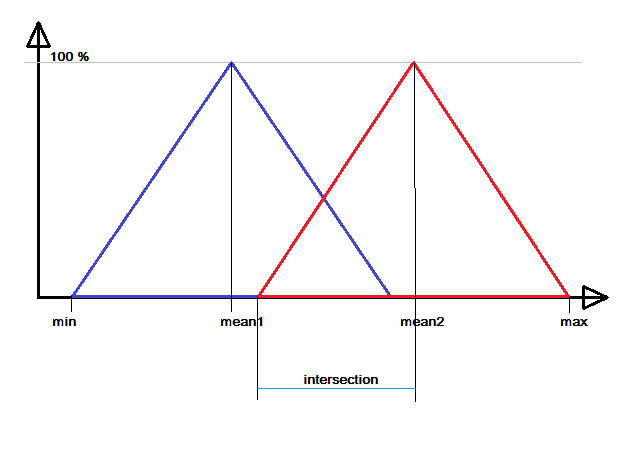
\includegraphics[scale=0.7]{images/fuzzy-sets.png}
	\caption{Fuzzy sets}
	\label{fig:fuzzy-sets}
\end{figure}

\subsubsection{Fuzzy sets construction}
So we have to construct two fuzzy sets from 4 feature values. In addition, for each feature is necessary determine $min$ and $max$ values. Each set represented as a triangle. At the top of the triangle membership probability is equal to 100\%. 

Algorithm is as follows:

\begin{enumerate}
	\item Sort values of feature
	\item $mean1=$ average value of two first numbers, $mean2=$ average value of two last numbers
	\item $intersection=$ 20\% of maximum element (first element)
	\item first set is= $\{ (min,0) , (mean1, 100) , (mean2-intersection, 0) \}$, second set is= $\{ (mean1+intersection, 0), (mean2, 100) , (max, 0) \}$
\end{enumerate}

Example with centroid values $\{580,3;519,54;359,08;350,02\}$\\
\[ sorting    \{580.3;519.54;359.08;350.02\} \]\\
\[ mean1=\frac{580.3+519.54}{2} \]
\[ mean2=\frac{359.08+350.02}{2}\]
\[intersection=\frac{580.3*20}{100}\]

Now is necessary define $min$ and $max$ values of this feature. Centroid is the center of mass for spectrum. Spectrum is representation of signal in frequency domain. And because fundamental frequency of human voice approximately  located between 30 and 1000 Hz. $min$ values for centroid is 30 and $max$ is 1000.

All features related with frequency range have such min and max values:
\begin{itemize}
	\item PitchDiff
	\item F1Dif, F2Dif, F3Dif
	\item PitchRange
	\item Centroid
\end{itemize}
For other features' $min$ and $max$ values was set on the basis of the spread of the values.

Eventually, we have got 5 values for two fuzzy sets construction. For each feature we can define two characterizing functions: $IsLow$ and $IsHigh$, which will return probability. And based on this model from training data set each emotion can be described as in the Table 4. So, accuracy of classification depends on properly selected fuzzy sets boundaries.


\begin{table}[h]
	\centering
		\begin{tabular}{l|l|l|l|l|}
			\hline
				Feature/Emotion& anger&	happy	&sadness	&neutral\\ \hline
PitchDff&	High	&High	&Low	&Low\\ \hline 
PitchDis&	High	&Low&	Low&	High\\ \hline
IntDif&	High&	High&	Low&	Low\\ \hline
IntDis	&High	&Low&	Low&	High\\ \hline
F1Dif&	High&	High&	Low&	Low\\ \hline
F1Dis&	High	&Low&	Low&	High\\ \hline
F2dif	&High&	Low&	High&	Low\\ \hline
F2Dis&	High&	Low&	Low	&High\\ \hline
F3Dif&	Low&	Low&	High&	High\\ \hline
F3Dis&	Low	&Low&	High&	High\\ \hline
PitchRange&	High&	High&Low&	Low\\ \hline
IntRange&	High&	High&	Low&	Low\\ \hline
PitchVariance&	High&	High&Low&	Low\\ \hline
IntVariance	&High&	High&	Low	&Low\\ \hline
PhraseDuration&	Low&	High&	High	&Low\\ \hline
SilenceDuration	&Low	&Low	&High&	High\\ \hline
Centroid&	High	&High&	Low&	Low\\ \hline
 \hline
		\end{tabular}
	\caption{}
	\label{tab:}
\end{table}

And the emotion probability computing will look like:\\ $anger=PitchDif.IsHigh() + PitchDis.IsLow() + IntDif.IsHigh() + ...$

So this classifier is obtained similar to Binary decision tree but with fuzzy logic. Both have simple implementation, fast classification, fast learning, make changes after learning is possible.
\subsection{System as whole}

\begin{figure}[h]
	\centering
		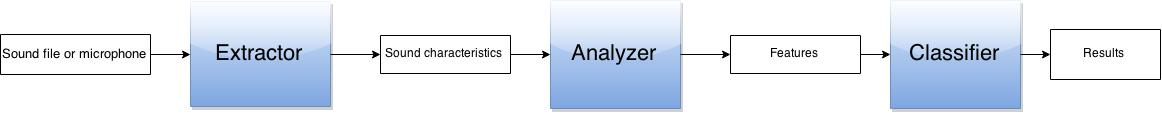
\includegraphics[scale=0.3]{images/components.png}
	\caption{System as a whole}
	\label{fig:system}
\end{figure}

System's work as whole shown in the Figure 7. Extractor receives sound from file or microphone and extracts sound characteristics using PRAAT. Then Analyzer computes features for sound characteristics for further classification. Classifier using fuzzy sets computes probability for each emotion.

\section{Testing}
Before considering the results of our implementation, is necessary to note some points about on what depends accuracy. As mentioned above, accuracy of the system depends on used features and classifier. But also it depends on training data set and data set used to test. Because there is real ambiguity between expressed emotions. Furthermore, EmoDB contains only artificially expressing emotions. So, some actors can express emotions ambiguously. More dependent on talk context and on person specific manner of speaking. It can be proved by results of human performance in emotion recognition (Figure 8) from \cite{frankthomas} paper.
\begin{figure}[h]
	\centering
	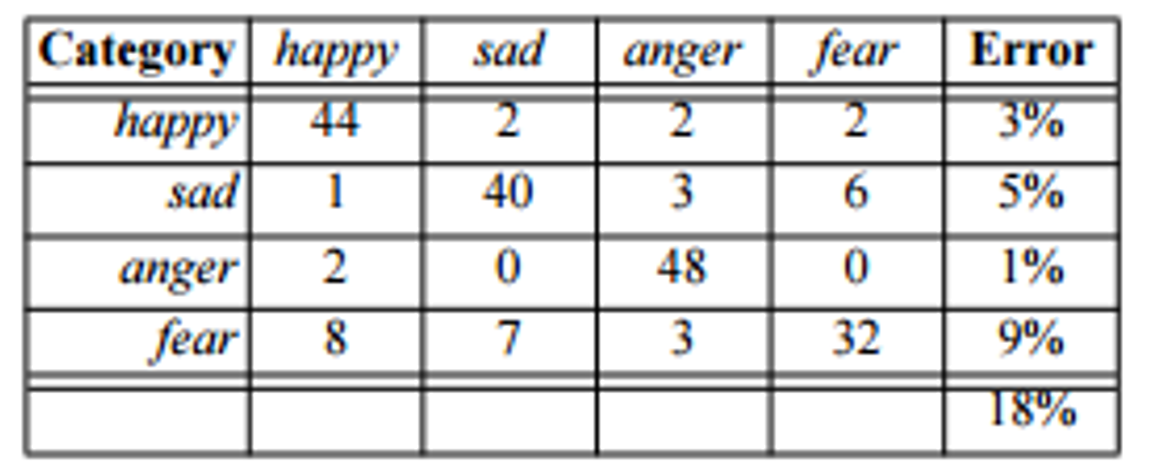
\includegraphics[scale=0.3]{images/h_performance.png}
	\caption{}
	\label{fig:human-perforance}
\end{figure}

\subsection{Results}
As noted above data set was divided into two parts: for training and testing. Here are results of testing using other part of data set.\\
\begin{table}[h]
	\centering
	\begin{tabular}{|l|l|l|l|l|}
		\hline
		&anger&happy&sadness&neutral\\ \hline
		anger&\textbf{55}&16&9&18\\\hline
		happy & 17 & \textbf{47} & 11 & 23 \\\hline
		sadness & 3 & 11 & \textbf{62} & 22\\\hline
		neutral & 20 & 15 & 15 & \textbf{51}\\\hline
		
	\end{tabular}
	\caption{Testing results}
\end{table}
\begin{table}[h]
	\centering
	\begin{tabular}{|l|l|l|l|}
		\hline
		&anger&happy&sadness\\ \hline
		anger&\textbf{54}&34&4\\\hline
		happy & 38 & \textbf{49} & 0\\\hline
		sadness & 10 & 0& \textbf{90}\\\hline
		
	\end{tabular}
	\caption{Testing results without neutral emotion.}
\end{table}
\begin{table}[h]
	\centering
	\begin{tabular}{|l|l|l|}
		\hline
		& active & passive\\ \hline
		active & \textbf{86} & 14\\\hline
		passive & 18 & \textbf{82}\\\hline
		
	\end{tabular}
	\caption{Testing results with active-passive emotions}
\end{table}
As we can see in the Table 5, the most precisely recognized sadness and anger, i.e. passive and active emotions. Table 6 where represented results without neutral emotions, shows that accuracy can be better. And neutral emotion can be deduced from analyzing other emotions values. For example, if values of anger, happiness and sadness are very close, it means that speech is neutral.


\section{Conclusions and further work}
According to the results of testing we can see: influence to accuracy have not only used features and classification methods, but also selected emotions for recognition. It confirms that recognizable emotions should be chosen specially for application domain of the system. For example, in some cases is needed only active-passive or positive-negative emotions recognition, and it can be more precise, as shown in testing results.

Of course, in our simple implementation wasn't used MFCC or other characteristic which can be useful. In addition, classification technique (some mix of Fuzzy sets and Binary decision tree) is not ideal, and for better results can be used another classificator.

But the main goal of this work in considering of studies and implementation solution. Our simple solution has some advantages and disadvantages:\\\\
\textit{Advantages:}
\begin{itemize}
	\item noise removing
	\item dividing speech to phrases
	\item fast learning (the main part of time spent for sound characteristics extraction, classifier learning is done very fast)
\end{itemize}
\textit{Disadvantages:}
\begin{itemize}
	\item accuracy is very strongly associated with training set. 
	\item dividing speech to phrases would be wrong with unfiltered noises
	\item fuzzy sets have $min$ and $max$ confines
\end{itemize}

\subsection{Further work}
So, for further work is necessary to consider these aspects: sound characteristics, features, classification and testing.

\subsubsection{Sound characteristics}
Besides pitch, loudness, formant can be used MFCC, or spectral characteristics. But is necessary to  make sure of need spectral characteristics, because it requires more time for calculating. That is why for speech recognition often used MFCC.

\subsubsection{Features}
Among of all features is necessary to select ones which have less dependence with person specifics, recording context. For universal using of the system they should describe speech signal dynamics. In addition, is necessary to find out the weight of each feature, in other words it's contribution to classification result.

\subsubsection{Classification and testing}
Further can be done:
\begin{itemize}
	\item classifier training with other training set and comparing results. There are many databases of emotional speech.
	\item use other classifier(k-NN, SVM, ANN) and compare accuracy
	\item classification to classes: postive-nagative, passive-active. Because it may be more precise
	\item try various combinations of classifier and set of emotions
\end{itemize}
\begin{thebibliography}{9}

\bibitem{affective}
"Affective computing",
http://en.wikipedia.org/wiki/Affective\_computing

\bibitem{pepper}
"Pepper",
https://www.aldebaran.com/en/a-robots/who-is-pepper

\bibitem{wiki1}
Fundamental frequency,
http://en.wikipedia.org/wiki/Fundamental\_frequency

\bibitem{wiki2}
Formant,
http://en.wikipedia.org/wiki/Formant

\bibitem{wiki3}
Mel-frequenc cepstrum
http://en.wikipedia.org/wiki/Mel-frequency\_cepstrum

\bibitem{wiki_loudness}
Sound loudness,
http://en.wikipedia.org/wiki/Loudness


\bibitem{SirishaSirvinasSiva}
"Speaker Emotion Recognition Based on Speech Features and Classification Techniques",
J. Sirisha Devi, Dr. Srinivas Yarramalle, Siva Prasad Nandyala\\
I.J. Computer Network and Information Security, 2014, 7, 61-77

\bibitem{brittaelizabet} "Real-time automatic emotion recognition
from speech",
 Dr. Britta Wrede, Prof. Dr. Elisabeth André, 2010

\bibitem{emodb}"EmoDB" Felix Burkhardt, Astrid Paeschke, Miriam Rolfes, Walter Sendlmeier und Benjamin Weiss
A Database of German Emotional Speech
Proceedings Interspeech 2005, Lissabon, Portugal\\
http://www.emodb.bilderbar.info/.

\bibitem{pierre}"The production and recognition of emotions in
speech: features and algorithms",
 Pierre-Yves Oudeyer,Int. J. Human-Computer Studies 59 (2003) 157–183

\bibitem{praat} "PRAAT",
 Paul Boersma and David Weenink   
Phonetic Sciences, University of Amsterdam//
http://www.fon.hum.uva.nl/praat/

\bibitem{frankthomas}"Recognizing emotion in speech",
Frank Dellaert, Thomas Polzin and Alex Waibel. Carnegie Mellon University. 


\end{thebibliography}
\end{document}
